\documentclass[12pt]{paper}
\usepackage{geometry}                % See geometry.pdf to learn the layout options. There are lots.
\geometry{letterpaper}                   % ... or a4paper or a5paper or ... 
%\geometry{landscape}                % Activate for for rotated page geometry
%\usepackage[parfill]{parskip}    % Activate to begin paragraphs with an empty line rather than an indent
\usepackage{graphicx}
\usepackage{amssymb}
\usepackage{epstopdf}
\usepackage{hyperref}
\usepackage{natbib}
\DeclareGraphicsRule{.tif}{png}{.png}{`convert #1 `dirname #1`/`basename #1 .tif`.png}

\newcommand{\aap}{{\it A\&A}}
%\newcommand{\aaps}{{\it A\&AS}}
\newcommand{\aj}{{\it AJ}}
\newcommand{\apj}{{\it ApJ}}
\newcommand{\apjl}{{\it ApJL}}
\newcommand{\mnras}{{\it MNRAS}}
\newcommand{\pasp}{{\it PASP}}

\title{Stellar Structure and Evolution Numerical Project}
\author{Samuel Factor}
%\date{}                                           % Activate to display a given date or no date

\begin{document}
\maketitle
%\section{}
%\subsection{}

Code for this project can be found at \\
\url{https://github.com/sfxfactor/StellarNumericalProj}.

\section{ZAMS and Starting Model}
Figure \ref{fig:fig1} is a reproduction of Figure 1 of \citet{BKL}. As I used the assumptions in the paper, and not real models, the curves are strait and not curved as in \citet{BKL}. I used two prescriptions for the effective temperature to see if it would bring the curves into better agreement with the curves in \citet{BKL}. One prescription was from Equation 6 of \citet{BKL} and the other was from the Eddington luminosity,
\begin{equation}\label{eq:tedd}
T_{eff}=\left(\frac{L_{edd}}{4\pi R^2 \sigma_{SB}}\right)^{1/4}.
\end{equation}


\begin{figure}
\begin{center}
    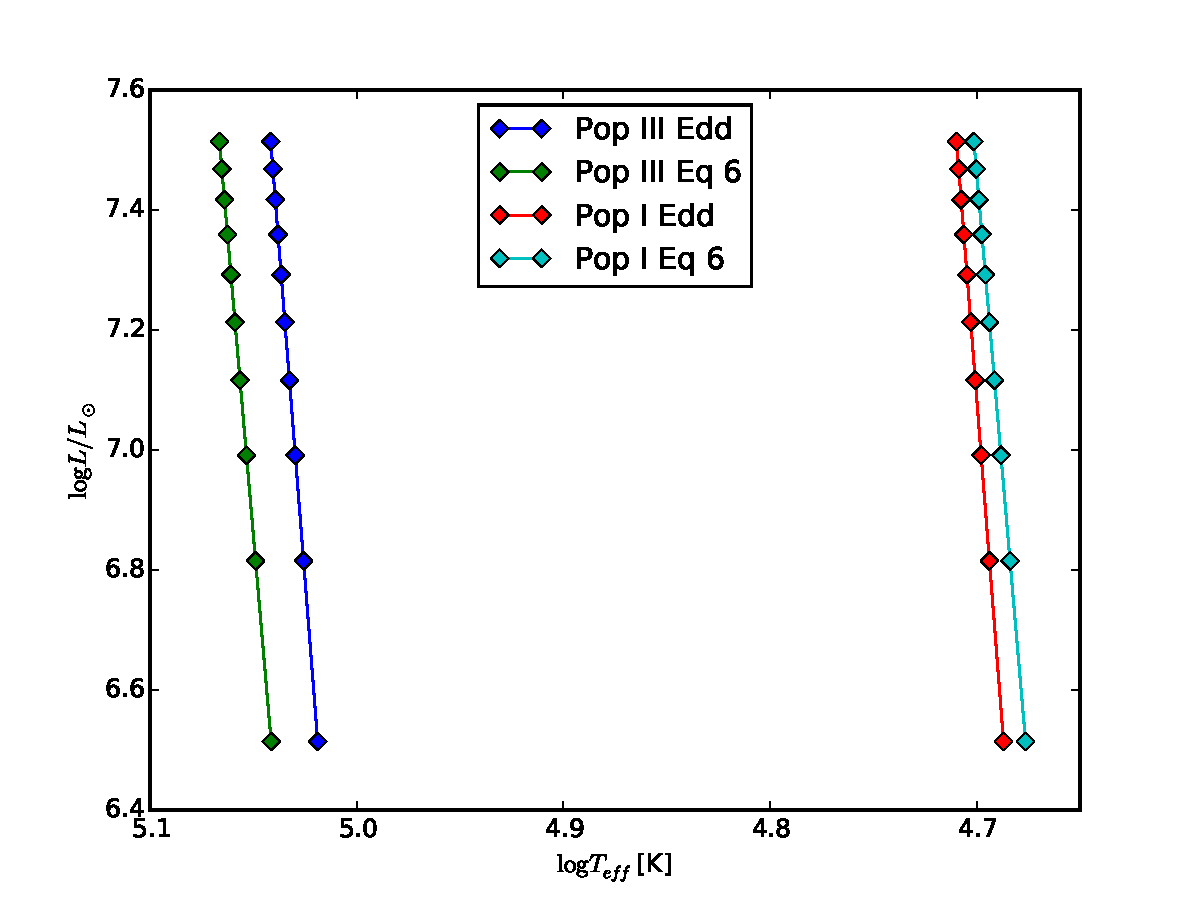
\includegraphics[width=0.6\textwidth]{fig1.pdf}
    \caption{HR Diagram for high mass ($M=100-1000~M_\odot$ in increments of $100~M_\odot$) Pop III (left) and Pop I (right) stars. Different curves correspond to temperatures given by Equation 6 of \citet{BKL} and the Eddington luminosity, Equation \ref{eq:tedd}. }
    \label{fig:fig1}
\end{center}
\end{figure}

Using my code from Problem Set 2, I generated an $n=3$ polytropic model of a $100M_\odot$ Pop III star. The pressure and density structure is shown in Figures \ref{fig:pm} and \ref{fig:dm} respectively. To calculate a temperature I assumed $\beta=0.58$. This value comes from Equation 19.56 in KW$^2$ 
\begin{equation}\label{eq:beta}
\frac{1-\beta}{\mu^4\beta^4}=3.02\times10^-3\left(\frac{M}{M_\odot}\right)^2.
\end{equation}
The temperature is then 
\begin{equation}\label{eq:temp}
T=\left((1-\beta)P\frac{3}{a}\right)^{1/4}
\end{equation}
This produces the temperature structure shown in Figure \ref{fig:tm}.

\begin{figure}
\begin{center}
    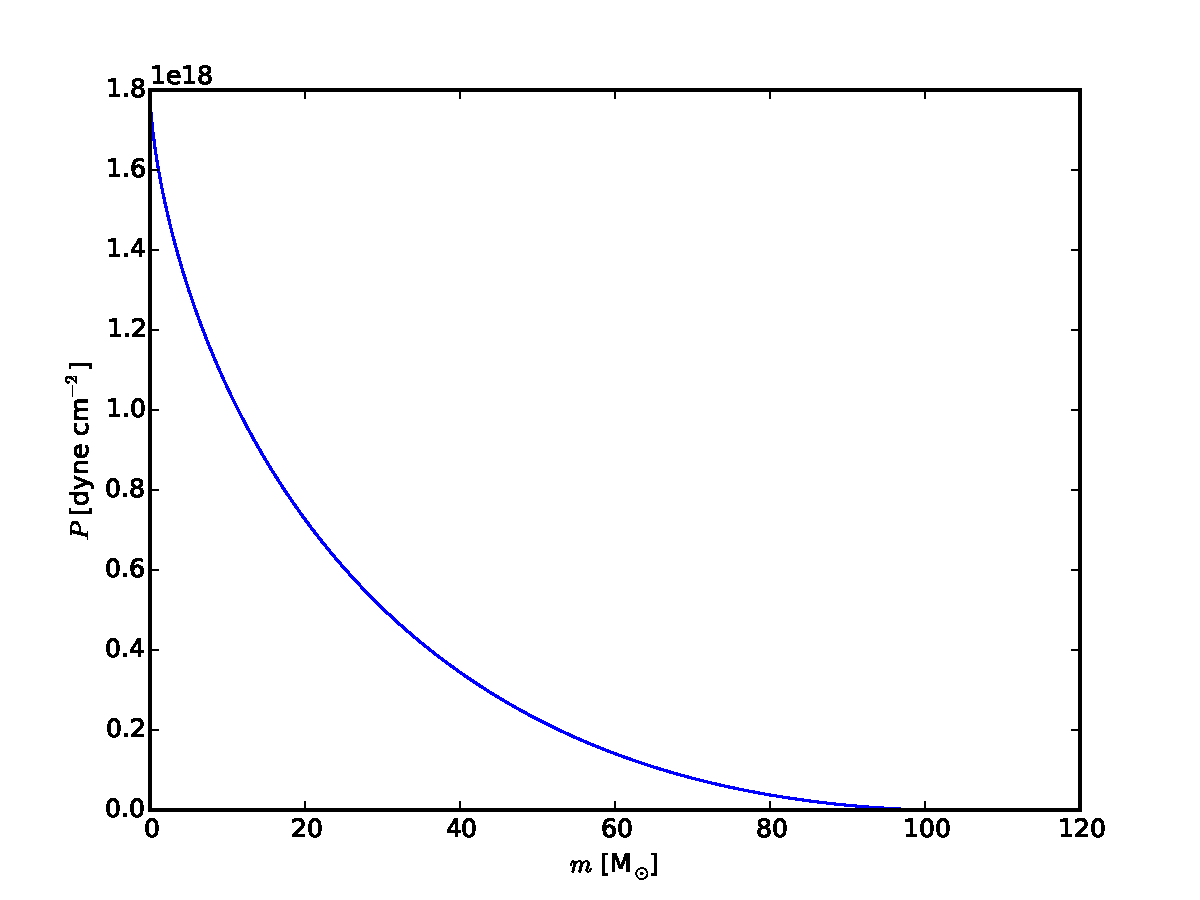
\includegraphics[width=0.6\textwidth]{pressure3p0.pdf}
    \caption{Pressure as a function of enclosed mass for an $n=3$ polytropic model of a $100~M_\odot$ Pop III star.}
    \label{fig:pm}
\end{center}
\end{figure}

\begin{figure}
\begin{center}
    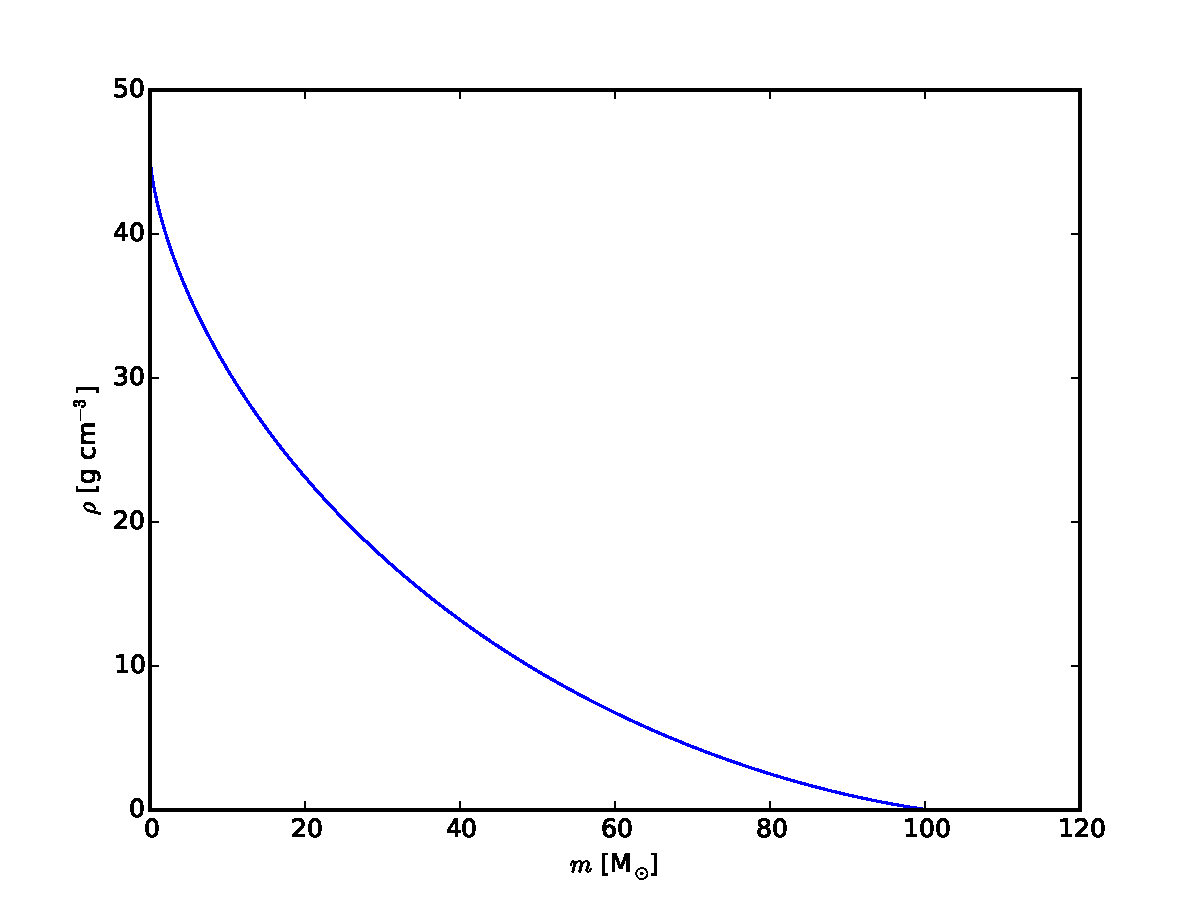
\includegraphics[width=0.6\textwidth]{density3p0.pdf}
    \caption{Density as a function of enclosed mass for an $n=3$ polytropic model of a $100~M_\odot$ Pop III star.}
    \label{fig:dm}
\end{center}
\end{figure}

\begin{figure}
\begin{center}
    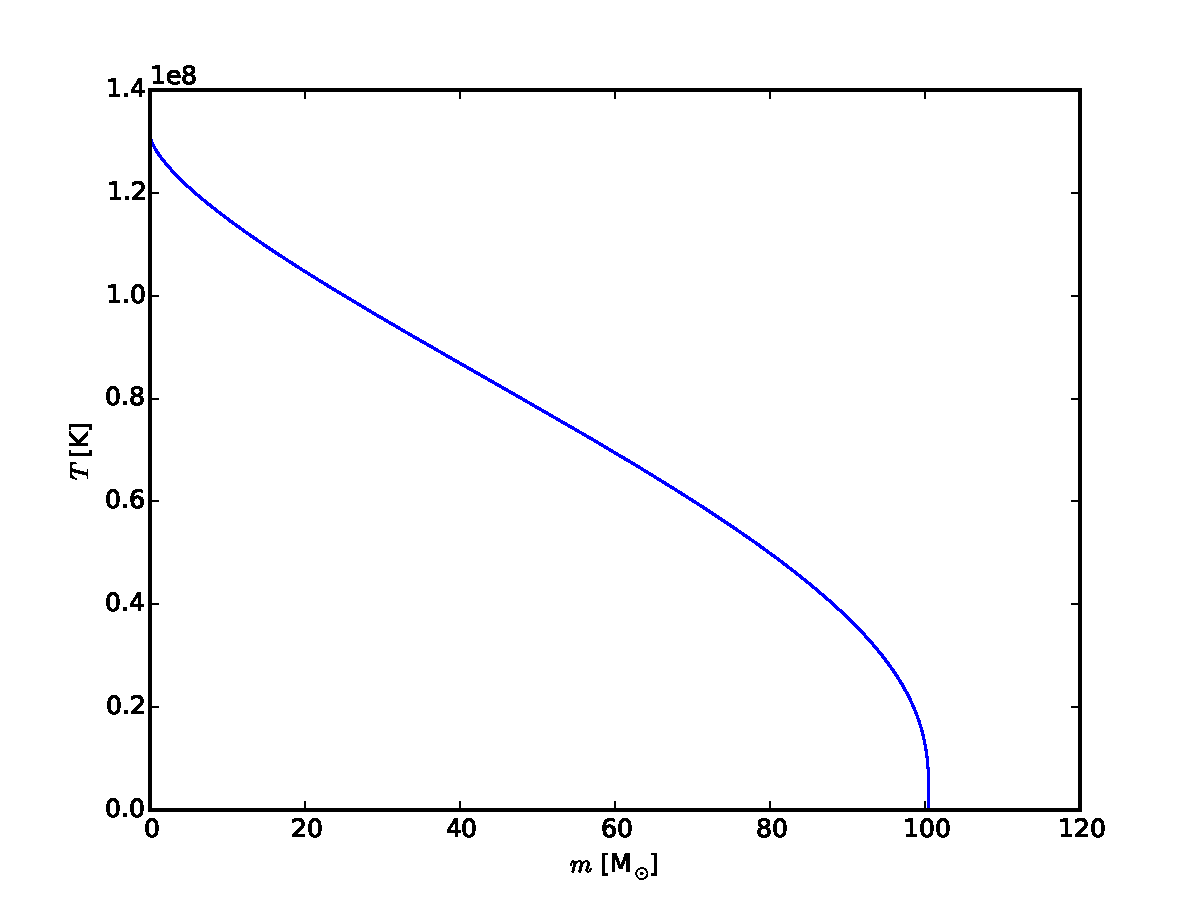
\includegraphics[width=0.6\textwidth]{temperature3p0.pdf}
    \caption{Temperature as a function of enclosed mass for an $n=3$ polytropic model of a $100~M_\odot$ Pop III star.}
    \label{fig:tm}
\end{center}
\end{figure}

\section{Evolving off the MS}
I worked together brielfy with Brianna and Ben on this part. 

I tried very hard to get the \texttt{STELLAR} code to work with a $100~M_\odot$ Pop III (metal free) star though was unsuccessful. You can see my commit history on GitHub to look at the specific changes I tried, but I will outline the important ones below. To see the specific changes I made, go to the link at the begining of this text and click on ``commits" in the top left. You can then click on each commit individually and GitHub will highlight the changes made. If you would rather I attach to this document a copy of the code with changes highlighted send me an email and I can do that. 

First, the initial conditions and polytropic index (in \texttt{polytr.inp}, \texttt{pmsstar.start}, \texttt{and pmsstar.inp}) and polytrope constants (in \texttt{polytr.F}) must be changed to match the $n=3$ $100~M_\odot$ metal free star we wish to model. I then changed the pressure prescription in \texttt{invstate.F} to fix $\beta$ at the value mentioned above (see Equation \ref{eq:beta}. Second I replaced all calls to \texttt{opacity} in \texttt{gi.F} with Thompson scattering opacity $0.2(1+X)$. In \texttt{atmos.F} I did the same thing but added H$^-$ opacity, $(1-X-Y)\rho^{1/2}T^9$. This was of course added in inverse according to $1/\kappa=1/\kappa_T+1/\kappa_{H^-}$. Finally I changed the luminosity prescription in \texttt{polytr.F} to Equation 3 of \citet{BKL}. 

When looking at the output of the failed stellar run I noticed that the energy generation predicted by the code from the CNO cycle was much too small ($\sim 10^7$ erg/s when the luminosity is $\sim10^{40}$). If this could be brought up the model may have converged. I probably could have changed this part of the code to simply use Equation 3 of \citet{BKL} but that may have effected the chemical evoultion.

If the 100 $M_\odot$ Pop III star would have evolved past the MS, the model would not have been able to model the pulsations caused by pair instability. This causes the rapid burning of oxygen and silicon, stopping the collapse with an enormous explosion. For stars $\sim 140-260 M_\odot$ \citep{pop3}this completely disrupts the star leaving behind no remnent. For masses less than this but greater than $\sim 100 M_\odot$ the pulsations throw off large amounts of mass while the core collapses into a black hole. This is what would probably happen to the star we are modeling.

Since I could not get the $100~M+\odot$ Pop III star to work, I modeled a few solar metalicity stars and tried to push their mass up as high as I could. Shown in Figure \ref{fig:HR} are evolution tracks for 1, 3, 4, 5, and 10 $M_\odot$ solar metalicity stars. You will notice that the 5 and 10 $M_\odot$ models fail when they reach the MS. The \texttt{STELLAR} code seems to be very sensitive to the initial $R$ and $T_{eff}$ of the polytrope model. For example, the initial $R$ and $T_{eff}$ of the 3 and 4 $M_\odot$ (which evolved past the MS) were almost identical. If I changed the 4 $M_\odot$ initial conditions a small amount, the star would evolve to the MS and the model would fail, much like the 5 and 10 $M_\odot$ models. 

\begin{figure}
\begin{center}
    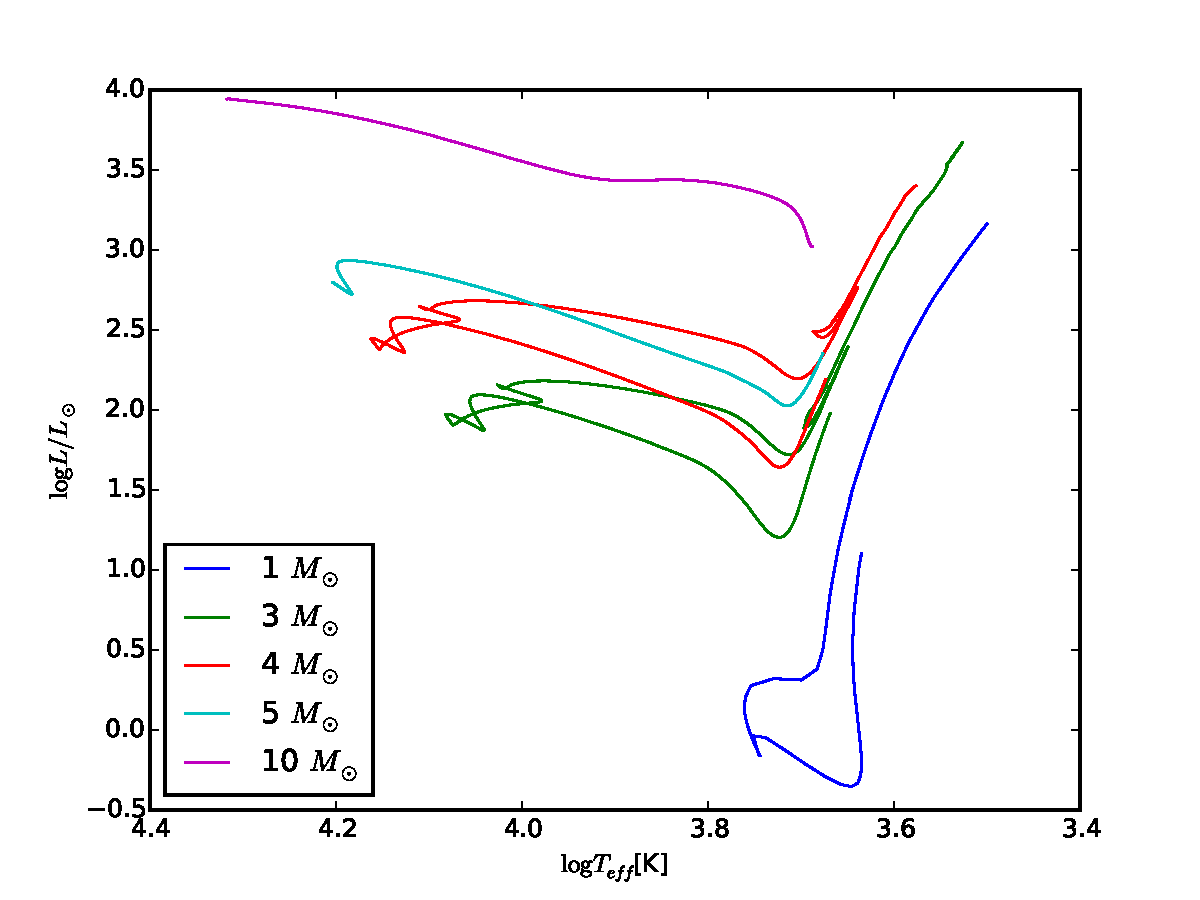
\includegraphics[width=\textwidth]{HR.pdf}
    \caption{Evolutionary tracks for solar metalicity stars. The two highest mass models fail when they reach the MS, while the lower mass models evolve off the MS. }
    \label{fig:HR}
\end{center}
\end{figure}

Figures \ref{fig:pse}, \ref{fig:dse}, and \ref{fig:tse} show the initial and final pressure, density, and temperature structures for the 4 $M_\odot$ model, the highest mass model that evolved off the MS.

\begin{figure}
\begin{center}
    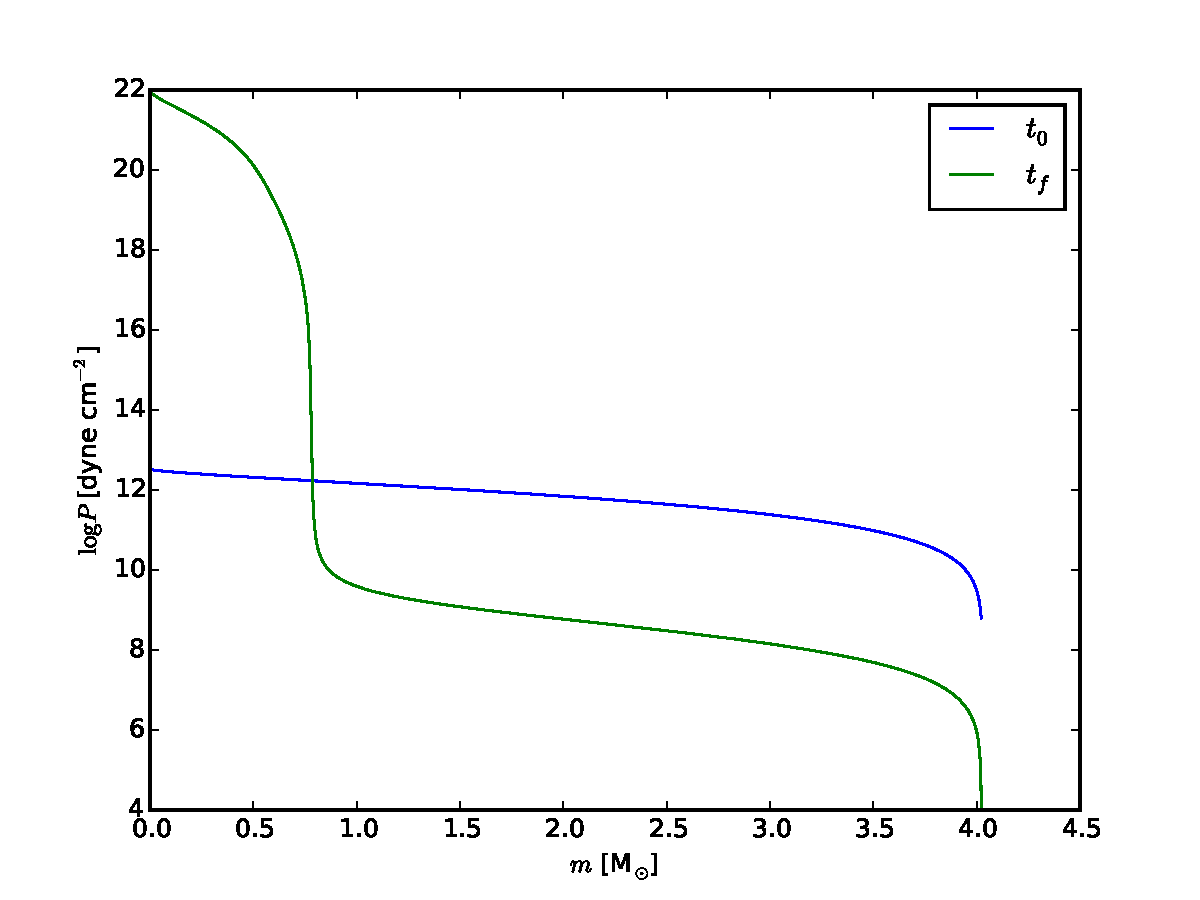
\includegraphics[width=0.6\textwidth]{pres.pdf}
    \caption{Pressure as a function of enclosed mass for a $4~M_\odot$ Pop I star at the beginning and end of its life.}
    \label{fig:pse}
\end{center}
\end{figure}

\begin{figure}
\begin{center}
    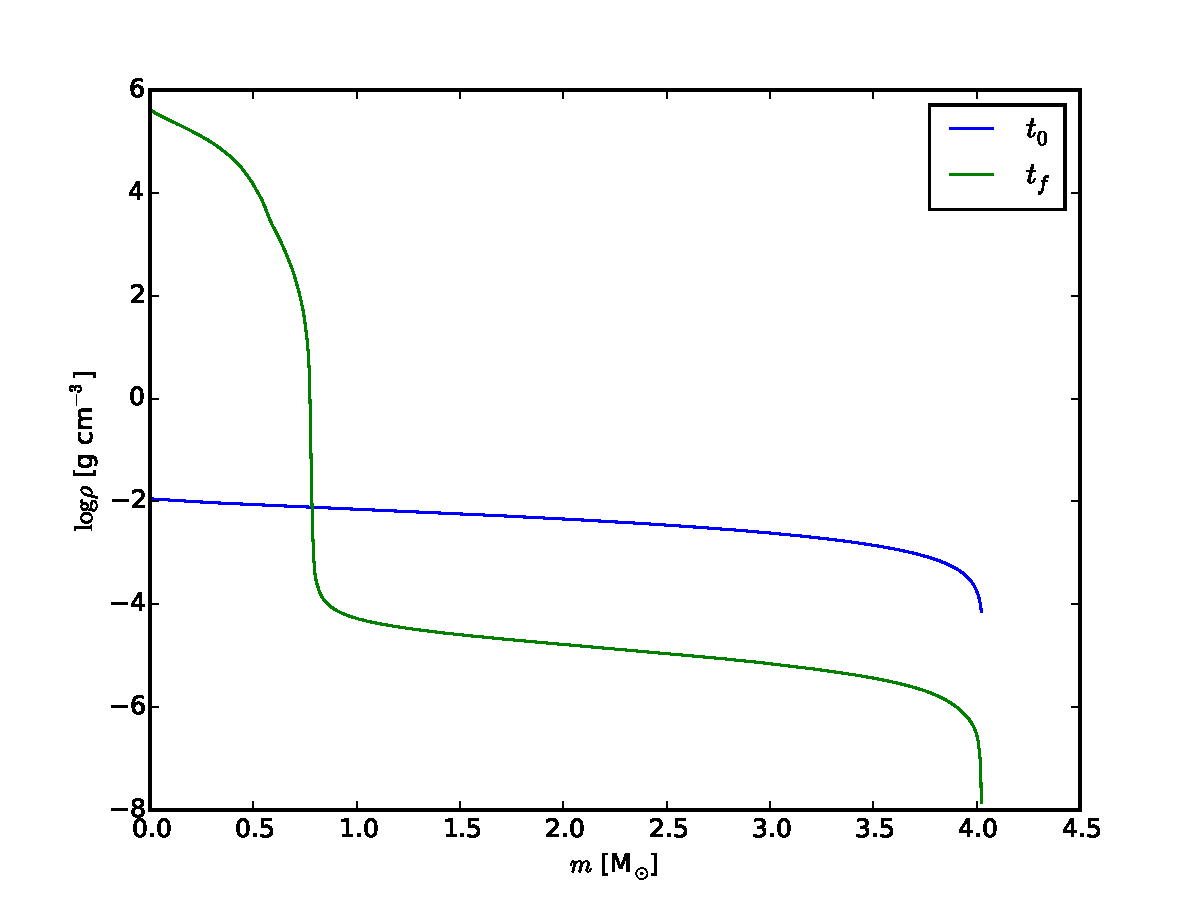
\includegraphics[width=0.6\textwidth]{dens.pdf}
    \caption{Density as a function of enclosed mass for a $4~M_\odot$ Pop I star at the beginning and end of its life.}
    \label{fig:dse}
\end{center}
\end{figure}

\begin{figure}
\begin{center}
    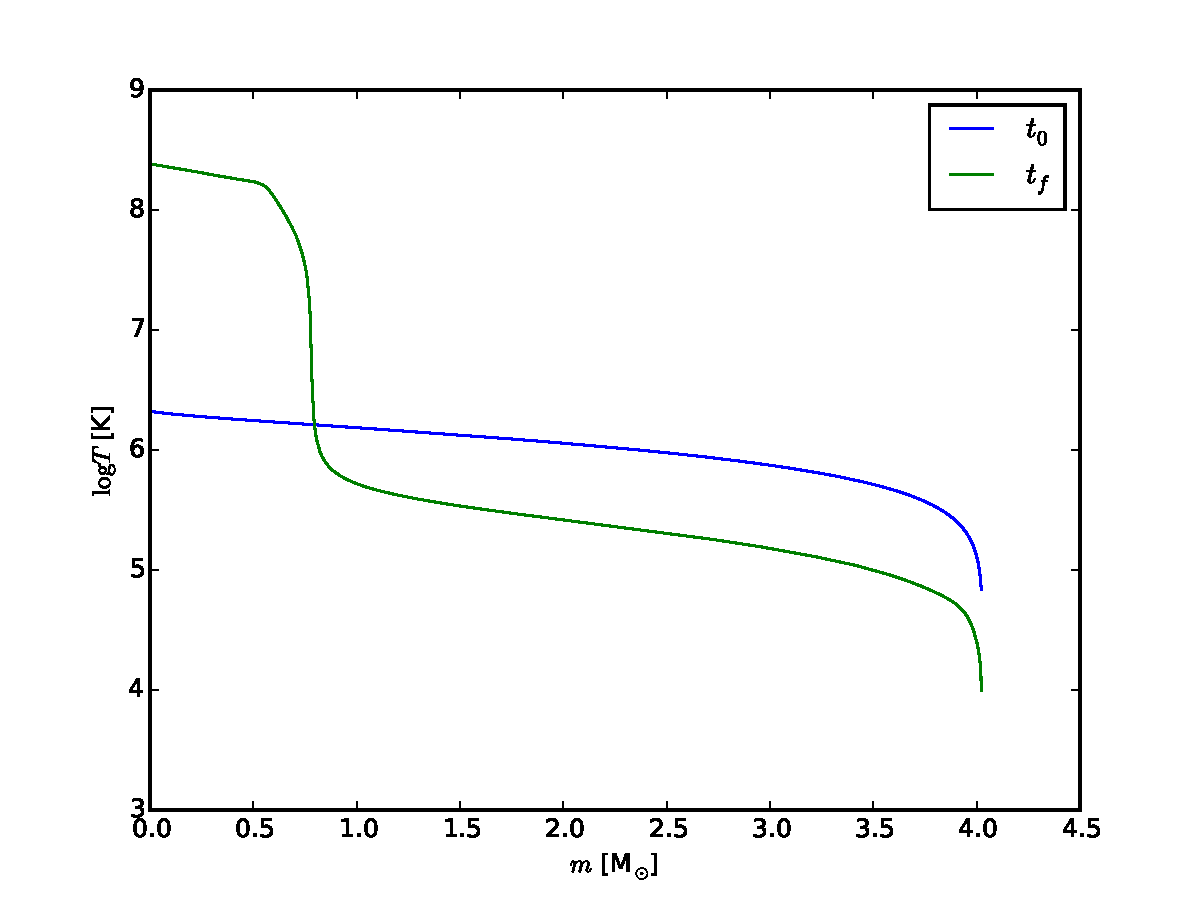
\includegraphics[width=0.6\textwidth]{temp.pdf}
    \caption{Temperature as a function of enclosed mass for a $4~M_\odot$ Pop I star at the beginning and end of its life.}
    \label{fig:tse}
\end{center}
\end{figure}

\setlength\bibsep{0pt}
\bibliographystyle{apj}
\bibliography{sources}
\end{document}  
